\documentclass[11pt]{article}

\usepackage[a4paper,margin=1in]{geometry}
\usepackage{amsmath,amssymb,mathtools}
\usepackage{authblk}
\usepackage{hyperref}

\usepackage{microtype}
\microtypesetup{expansion=false}
\usepackage{physics}
\usepackage{enumitem}
\usepackage{graphicx}
\usepackage{booktabs}
\usepackage{listings}
\usepackage{xcolor}

\hypersetup{
    colorlinks=true,
    linkcolor=blue,
    citecolor=blue,
    urlcolor=blue
}

% ---------- Minimal notation (self-contained) ----------
\newcommand{\vswirl}{\mathbf{v}_{\!\boldsymbol{\circlearrowleft}}} % characteristic swirl speed (model parameter)
\newcommand{\vnorm}{\lVert \vswirl \rVert}
\newcommand{\rhof}{\rho_{\!f}}
\newcommand{\rhoE}{\rho_{\!E}}
\newcommand{\rhoM}{\rho_{\!m}}

\newcommand{\Sinfo}{S_{\mathrm{info}}}
\newcommand{\Ta}{T_a}
\newcommand{\Tmu}{T_\mu}
\newcommand{\chia}{\partial_a \chi}
\newcommand{\tauone}{\boldsymbol{\tau}}   % the 1-form symbol (optional)
\newcommand{\taucomp}[1]{\tau_{#1}}       % component macro
\newcommand{\Omab}{\Omega_{ab}}
\newcommand{\Omuv}{\Omega_{\mu\nu}}
\newcommand{\tua}{\tau_a}


\lstset{
    basicstyle=\ttfamily\small,
    keywordstyle=\color{blue},
    commentstyle=\color{gray},
    stringstyle=\color{teal},
    breaklines=true,
    frame=single,
    columns=fullflexible
}

\title{Informational Gradients as Local Time Fields:\\Dimensional Closure, Integrability, and Medium-Based Clock Mappings}
\author[1]{Omar Iskandarani}
\affil[1]{Independent Researcher}
\date{\today}

\begin{document}
    \maketitle

    \begin{abstract}
        A recent proposal formulates time as a local field defined by gradients of stored information, $\Ta(x)=\partial_a \Sinfo(x)$, and suggests that geometry can be linked to second derivatives of an informational potential \cite{Neukart2026_InfoTime}. This article develops a self-contained effective-field treatment of informational time with four aims: (i) enforce dimensional consistency by introducing an operational information-to-time calibration rate; (ii) clarify integrability by distinguishing exact time one-forms from connection-augmented non-integrable time fields with measurable holonomy; (iii) discuss how Hessian-type metric constructions relate to established information geometry and the constraints imposed by Lorentzian signature and covariance; and (iv) provide constructive toy models and simulation schemes on discrete lattices, together with falsifiable observational signatures in clock networks and long-baseline quantum coherence distribution. A medium-based ``swirl-clock'' mapping is presented as a constitutive option (without claiming equivalence to relativity unless a specific characteristic speed is identified with $c$), in the spirit of analogue-gravity methods.
    \end{abstract}

    \noindent\textbf{Keywords:} problem of time; informational time; entropy gradients; integrability; holonomy; information geometry; analogue gravity; clock networks


    \begin{figure}[t]
    \centering
    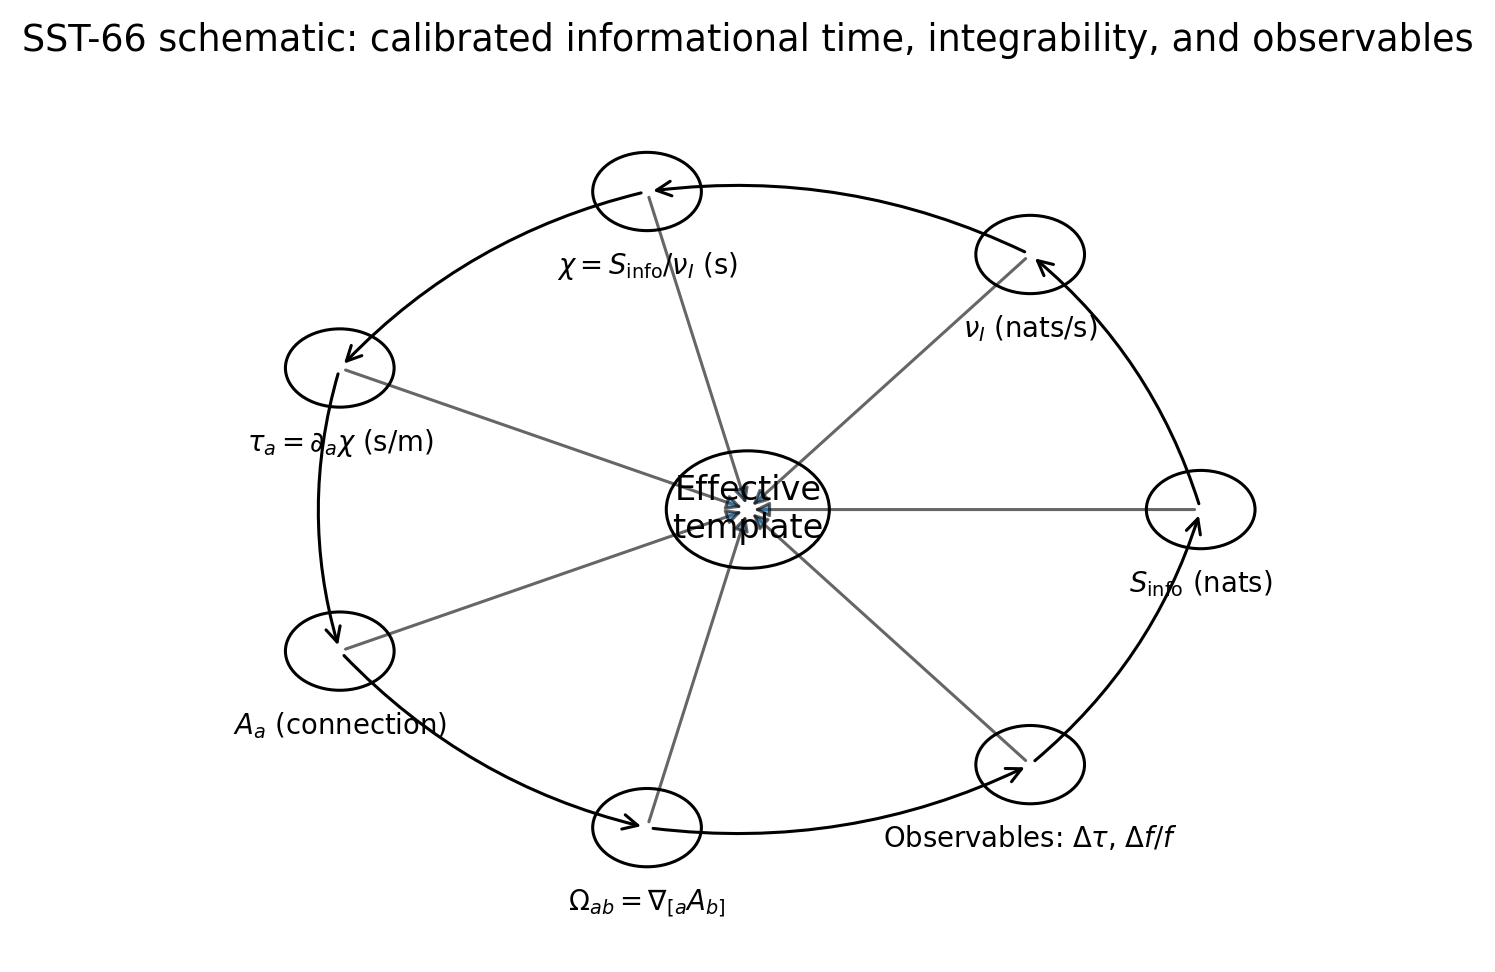
\includegraphics[width=\linewidth]{fig_sst66_v2_01_model_map.png}
    \caption{Schematic map of the effective “informational time” template: calibration from $S_{\mathrm{info}}$ to $\chi$, integrable one-form $\tau_a=\partial_a\chi$, optional connection $A_a$ with curvature $\Omega_{ab}$, and measurable observables such as loop time offsets.}
    \label{fig:model_map}
    \end{figure}


    \section{Motivation and scope}
        Time occupies incompatible roles across quantum mechanics and gravitation. In standard quantum mechanics, the Schr\"odinger equation treats time as an external parameter,
        \begin{equation}
            i\hbar \frac{\partial}{\partial t}\Psi(t)=\hat H \Psi(t),
            \label{eq:schro}
        \end{equation}
        while in general relativity (GR) time is part of a dynamical geometry \cite{Wald1984_GR}. In canonical quantum gravity, the Wheeler--DeWitt equation produces ``frozen'' dynamics with no explicit time parameter \cite{DeWitt1967_Canonical,Isham1993_ProblemTime,Kuchar1992_TimeInterp}. Relational approaches reconstruct time from correlations \cite{PageWootters1983_Evolution,Rovelli1991_TimeHypothesis}, and thermodynamic approaches attempt to relate time's arrow to entropy growth \cite{Lebowitz1993_Boltzmann,ConnesRovelli1994_ThermalTime}.

        Neukart proposes a different angle: time arises as a \emph{local informational field} rather than a universal coordinate, defining a temporal direction by gradients of stored information \cite{Neukart2026_InfoTime}. The present paper does not assume a specific microscopic substrate (such as a Planck-lattice ``memory matrix''). Instead, it extracts a minimal effective-field template and makes it precise enough to be internally consistent and testable.

        We emphasize two distinctions:
        \begin{enumerate}[label=(\roman*)]
\item \textbf{Operational vs ontological.} A time field should be defined via observables (clock readouts, phase accumulation, network synchronization) rather than metaphysical claims.
\item \textbf{Integrable vs non-integrable time.} If time is a gradient of a scalar potential, it is locally curl-free; if ``temporal curl'' is allowed, it must be modeled by additional structure (defects, discreteness, or a connection).
        \end{enumerate}

    \section{Informational time as a gradient field}
        \subsection{The gradient ansatz}
            The core construction is to posit a scalar ``informational potential'' $\Sinfo(x)$ and define a covector (one-form)
            \begin{equation}
                \Ta(x) = \partial_a \Sinfo(x).
                \label{eq:Ta_def}
            \end{equation}
            In Neukart's work, $\Sinfo$ is interpreted as a coarse-grained measure of stored information (e.g., a von Neumann entropy of a reduced density matrix) and $\Ta$ defines the local temporal direction \cite{Neukart2026_InfoTime}. Similar themes appear in ``thermal time'' (time from modular flow of a state) \cite{ConnesRovelli1994_ThermalTime} and in entropic gravity discussions \cite{Jacobson1995_ThermoSpacetime,Verlinde2011_Entropic}.

            However, \eqref{eq:Ta_def} as written is not dimensionally complete (since $\Sinfo$ is dimensionless), and it is automatically locally integrable (curl-free). Both issues must be addressed to turn the ansatz into a consistent effective theory.

        \subsection{Dimensional closure: from information to seconds}
            Let $\Sinfo$ be measured in \emph{nats} (dimensionless). Then $\partial_a\Sinfo$ has units of inverse length.
            Introduce an operational calibration rate $\nu_I$ with units nats/s and define a dimensionful scalar time potential
            \begin{equation}
                \chi(x) := \frac{1}{\nu_I}\, \Sinfo(x),
                \qquad [\chi]=\mathrm{s}.
                \label{eq:chi_def}
            \end{equation}
            Define the \emph{time one-form}
            \begin{equation}
                \tua := \partial_a \chi = \frac{1}{\nu_I}\,\partial_a \Sinfo,
                \qquad [\tua]=\mathrm{s/m}.
                \label{eq:tua_def}
            \end{equation}
            Along a worldline $x^\mu(\lambda)$, define informational proper time increments by line integration:
            \begin{equation}
                d\tau_I := \tua \, dx^a = \frac{1}{\nu_I}\,\partial_\mu \Sinfo\,dx^\mu.
                \label{eq:tauI_line}
            \end{equation}
            This makes the operational content explicit: $\nu_I$ is fixed by the clock modality (event-counting, irreversible updates, decoherence events, etc.). It is not a new fundamental constant; it is a calibration parameter, analogous in spirit to coarse-graining choices in statistical mechanics \cite{CoverThomas2006_InfoTheory,Lebowitz1993_Boltzmann}.

            \begin{figure}[t]
                \centering
                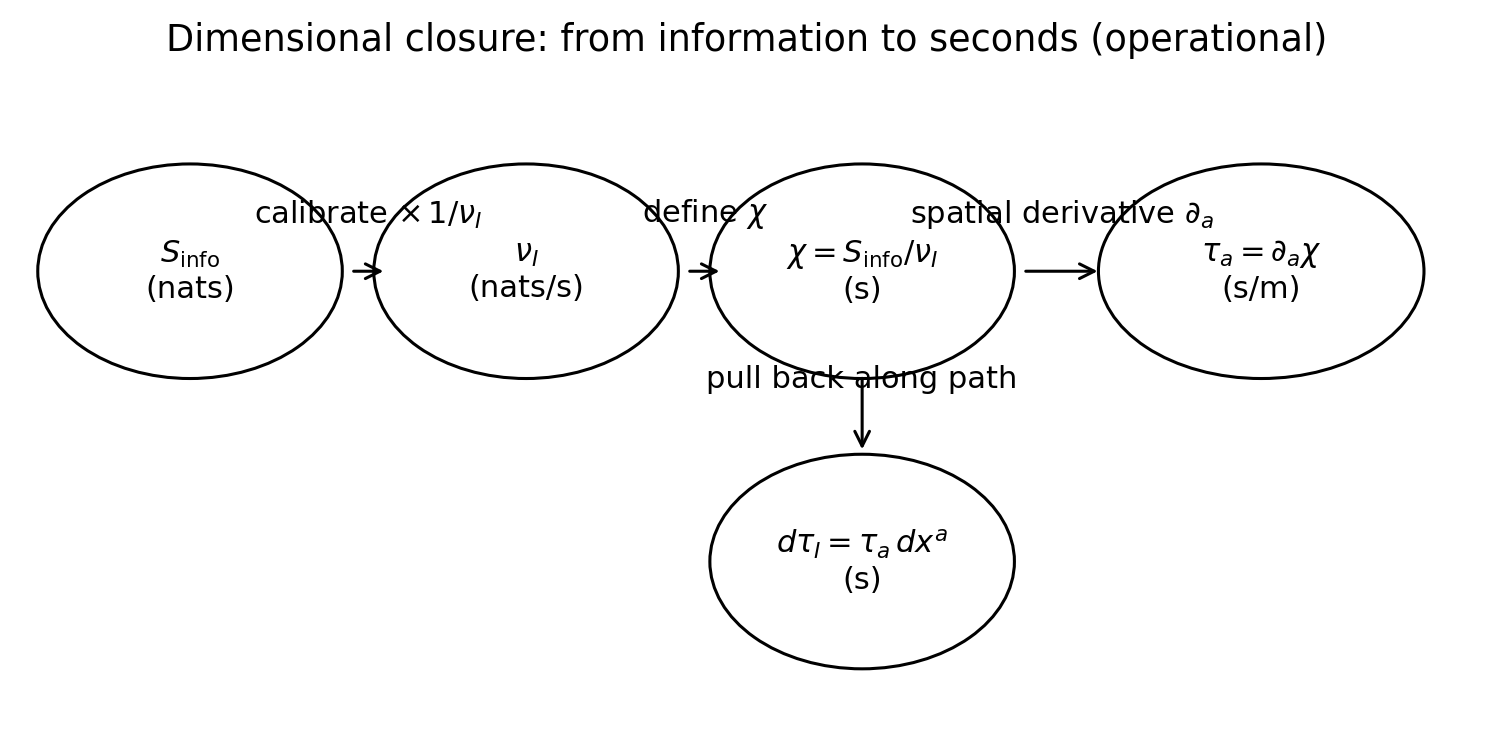
\includegraphics[width=\linewidth]{fig_sst66_v2_02_dimensional_closure.png}
                \caption{Dimensional closure from information to seconds: $S_{\mathrm{info}}$ (nats) calibrated by $\nu_I$ (nats/s) defines $\chi$ (s), whose gradient yields $\tau_a$ (s/m), and whose pullback gives $d\tau_I=\tau_a\,dx^a$.}
                \label{fig:dimensional_closure}
            \end{figure}

        \subsection{What does ``time dilation'' mean here?}
            If clocks measure accumulated $\tau_I$ and if $\tua$ varies across space, then two clocks at different locations can exhibit different rates due to different values of invariants built from $\chi$:
            \begin{equation}
                \text{clock rate} \;\sim\; \frac{d\tau_I}{dt_{\rm ref}}
                \;=\; \tua u^a,
                \label{eq:rate_general}
            \end{equation}
            where $u^a=dx^a/dt_{\rm ref}$ is the observer's tangent in a chosen reference coordinate. This is not yet GR: GR time dilation is geometric (metric-based). Here it is ``potential-based'' and becomes GR-like only if $\chi$ is tied consistently to an effective metric or to the physical mechanisms that set clock frequencies. That mapping is where model content lives.

    \section{Integrability, holonomy, and the meaning of ``temporal curl''}
        \subsection{Exact one-forms are locally curl-free}
            If $\tua=\partial_a\chi$ with smooth $\chi$, then
            \begin{equation}
                \nabla_{[a}\tua_{b]} = 0
                \quad\text{(locally)}.
                \label{eq:poincare}
            \end{equation}
            This is a standard result: exact one-forms are closed (Poincar\'e lemma) \cite{Frankel2011_GeometryPhysics,BottTu1982_DiffForms,Nakahara2003_Geometry}. Therefore, if a model wishes to allow a nonzero antisymmetric derivative $\nabla_{[a}\tua_{b]}\neq 0$, it must specify how exactness is broken.

        \subsection{Connection-augmented time and measurable holonomy}
            A clean mechanism is to introduce a time connection $A_a$ and define
            \begin{equation}
                \tua = \partial_a\chi + A_a.
                \label{eq:tua_conn}
            \end{equation}
            Define the associated curvature (a two-form)
            \begin{equation}
                \Omab := \nabla_a\tua_b-\nabla_b\tua_a = \nabla_aA_b-\nabla_bA_a.
                \label{eq:Omega_def}
            \end{equation}
            Now ``temporal curl'' is represented by $\Omab$, and it is measurable via holonomy around loops:
            \begin{equation}
                \Delta\tau_{\rm loop} \;:=\; \oint \tua\,dx^a
                \;=\; \oint A_a\,dx^a
                \;=\; \int_{\Sigma} \Omab\, d\Sigma^{ab},
                \label{eq:stokes}
            \end{equation}
            where $\Sigma$ spans the loop (Stokes' theorem) \cite{Frankel2011_GeometryPhysics,Nakahara2003_Geometry}. This is directly analogous in mathematics to gauge holonomy (e.g., Aharonov--Bohm phase), though the observable here is a \emph{time offset} rather than an electromagnetic phase \cite{AharonovBohm1959_AB}.

            \paragraph{Interpretation.}
                If $A_a=0$, time is locally integrable and can be parameterized by a scalar potential $\chi$ on simply-connected patches. If $A_a\neq0$, the time field is non-integrable, and loop-dependent time offsets become possible in principle.

            \begin{figure}[t]
                \centering
                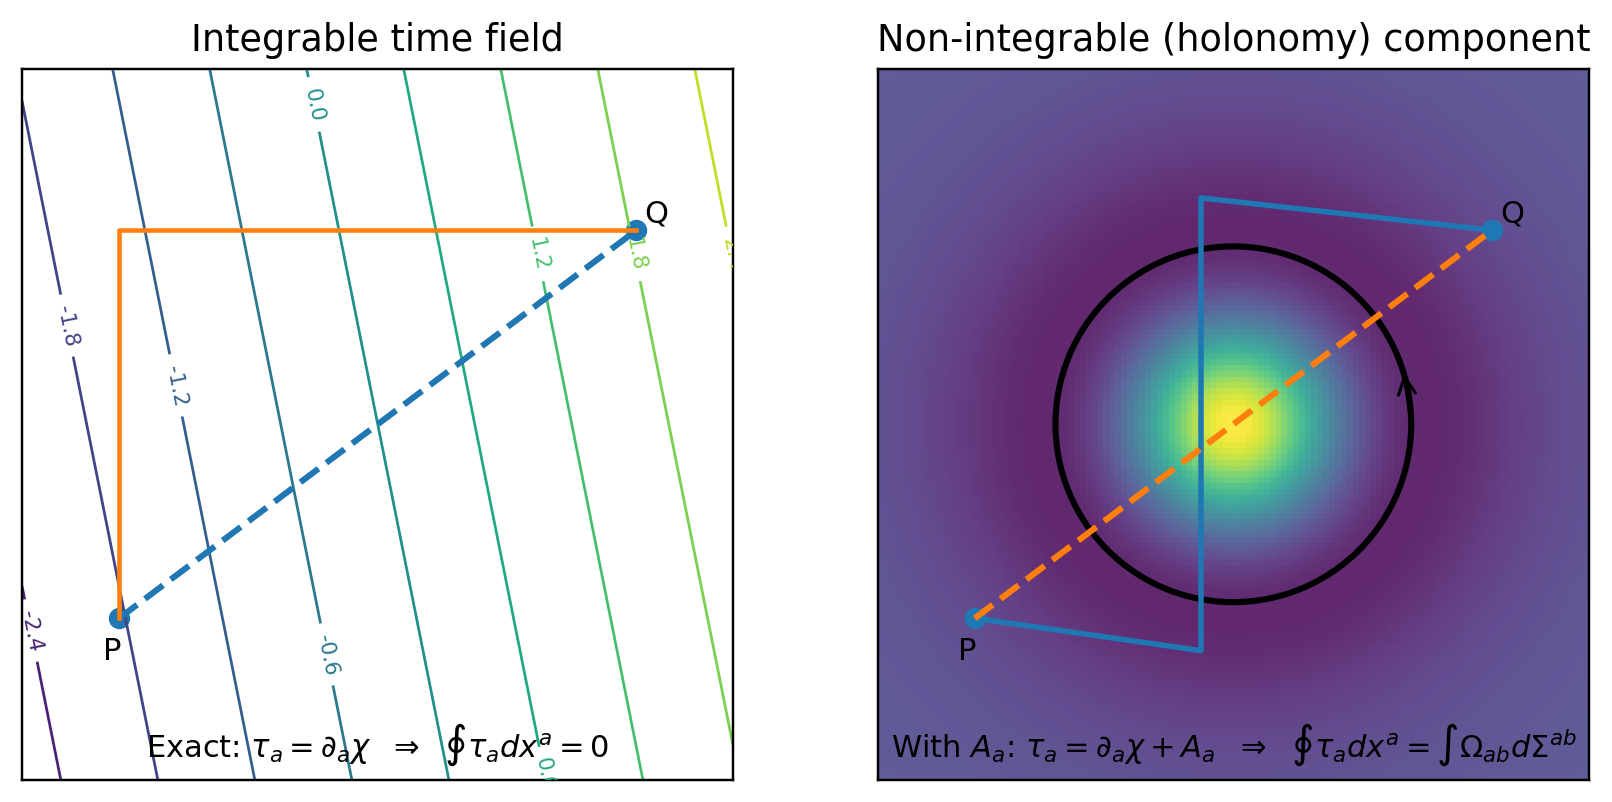
\includegraphics[width=\linewidth]{fig_sst66_v2_03_integrability_holonomy.png}
                \caption{Integrable vs non-integrable time. Left: if $\tau_a=\partial_a\chi$, then $\oint \tau_a dx^a=0$ on simply connected domains. Right: adding a connection $A_a$ permits holonomy, with loop offsets $\oint \tau_a dx^a=\int_\Sigma \Omega_{ab}\,d\Sigma^{ab}$.}
                \label{fig:integrability_holonomy}
                \end{figure}

    \subsection{Discrete lattices and effective non-commutativity}
        In discrete update systems (lattices, graphs), ``curl'' can appear even when a scalar potential exists, because discrete derivatives do not necessarily commute and defects can create topological obstructions. In practice, one can still decompose the discrete field into gradient and rotational parts (a discrete Helmholtz decomposition) and interpret the rotational part as an effective connection term \cite{LeVeque2002_FVM,Press2007_NR}.

    \section{Geometry from information: Hessian metrics and constraints}
    \subsection{Hessian constructions in information geometry}
        Information geometry equips families of probability distributions with Riemannian metrics derived from convex potentials; the Fisher information metric is central \cite{Amari2016_InfoGeometry,CoverThomas2006_InfoTheory}. More generally, Hessian metrics can be defined from a potential $\Phi$ by
        \begin{equation}
            g_{ij} = \partial_i\partial_j \Phi,
            \label{eq:hessian_metric}
        \end{equation}
        typically yielding positive-definite metrics in the appropriate coordinate systems.

        Neukart sketches a relation $g_{\mu\nu}\propto \partial_\mu\partial_\nu \Sinfo$ \cite{Neukart2026_InfoTime}. Interpreting this as a Lorentzian spacetime metric faces obstacles:
        \begin{enumerate}[label=(\alph*)]
\item \textbf{Signature.} A Hessian is not generically Lorentzian; additional structure is required to ensure one negative eigenvalue.
\item \textbf{Covariance.} Partial derivatives of a scalar are tensors, but Hessians depend on connection choice when expressed covariantly; defining geometry from second derivatives can be circular if the connection depends on $g_{\mu\nu}$.
\item \textbf{Uniqueness.} Many metrics can share the same local ``potential curvature'' up to transformations.
        \end{enumerate}
        These do not invalidate the idea; they constrain how it should be formulated.

    \subsection{A conservative, covariant alternative}
        Rather than defining $g_{\mu\nu}$ as a Hessian directly, treat $\chi$ as an additional physical field on an existing Lorentzian manifold and let it \emph{source} geometry through its stress--energy, as in scalar-field gravity:
        \begin{equation}
            S[g,\chi] = \int d^4x\sqrt{-g}\left[\frac{R}{16\pi G} -\frac{\lambda}{2}(\nabla\chi)^2 - V(\chi)\right],
            \label{eq:action_scalar}
        \end{equation}
        with corresponding stress--energy tensor \cite{Wald1984_GR}
        \begin{equation}
            T_{\mu\nu}^{(\chi)} = \lambda\left(\nabla_\mu\chi\nabla_\nu\chi-\frac{1}{2}g_{\mu\nu}(\nabla\chi)^2\right) - g_{\mu\nu}V(\chi).
            \label{eq:Tmunu_scalar}
        \end{equation}
        This yields a mathematically standard, covariant framework. ``Geometry-information duality'' becomes an effective statement about how $\chi$ correlates with gravitational potentials, not an identity $g\sim \partial^2\chi$.

    \subsection{Optional twist dynamics}
        If non-integrable time is desired, include a Maxwell-type action for the curvature $\Omuv$:
        \begin{equation}
            S_{\Omega}[g,A] = -\frac{\zeta}{4}\int d^4x\sqrt{-g}\,\Omuv\Om^{\mu\nu},\qquad \Omuv=\nabla_\mu A_\nu-\nabla_\nu A_\mu.
            \label{eq:action_twist}
        \end{equation}
        This makes loop time offsets quantitatively predictive.

    \section{Toy models: continuous and discrete}
    \subsection{Continuous toy potential: localized ``information well''}
        Consider a static scalar profile in flat space:
        \begin{equation}
            \chi(\mathbf{x}) = \chi_0 + \Delta\chi\, e^{-r^2/(2\sigma^2)}.
            \label{eq:gauss}
        \end{equation}
        Then
        \begin{equation}
            \nabla\chi(\mathbf{x}) = -\Delta\chi\,\frac{\mathbf{x}}{\sigma^2}\,e^{-r^2/(2\sigma^2)},
            \qquad
            \|\nabla\chi\|^2 = \Delta\chi^2\,\frac{r^2}{\sigma^4}\,e^{-r^2/\sigma^2}.
            \label{eq:grad_gauss}
        \end{equation}
        Any clock-rate functional depending on $\|\nabla\chi\|$ (see \S\ref{sec:clockmap}) predicts spatially varying rates peaked around $r\sim \sigma$.

        \begin{figure}[t]
            \centering
            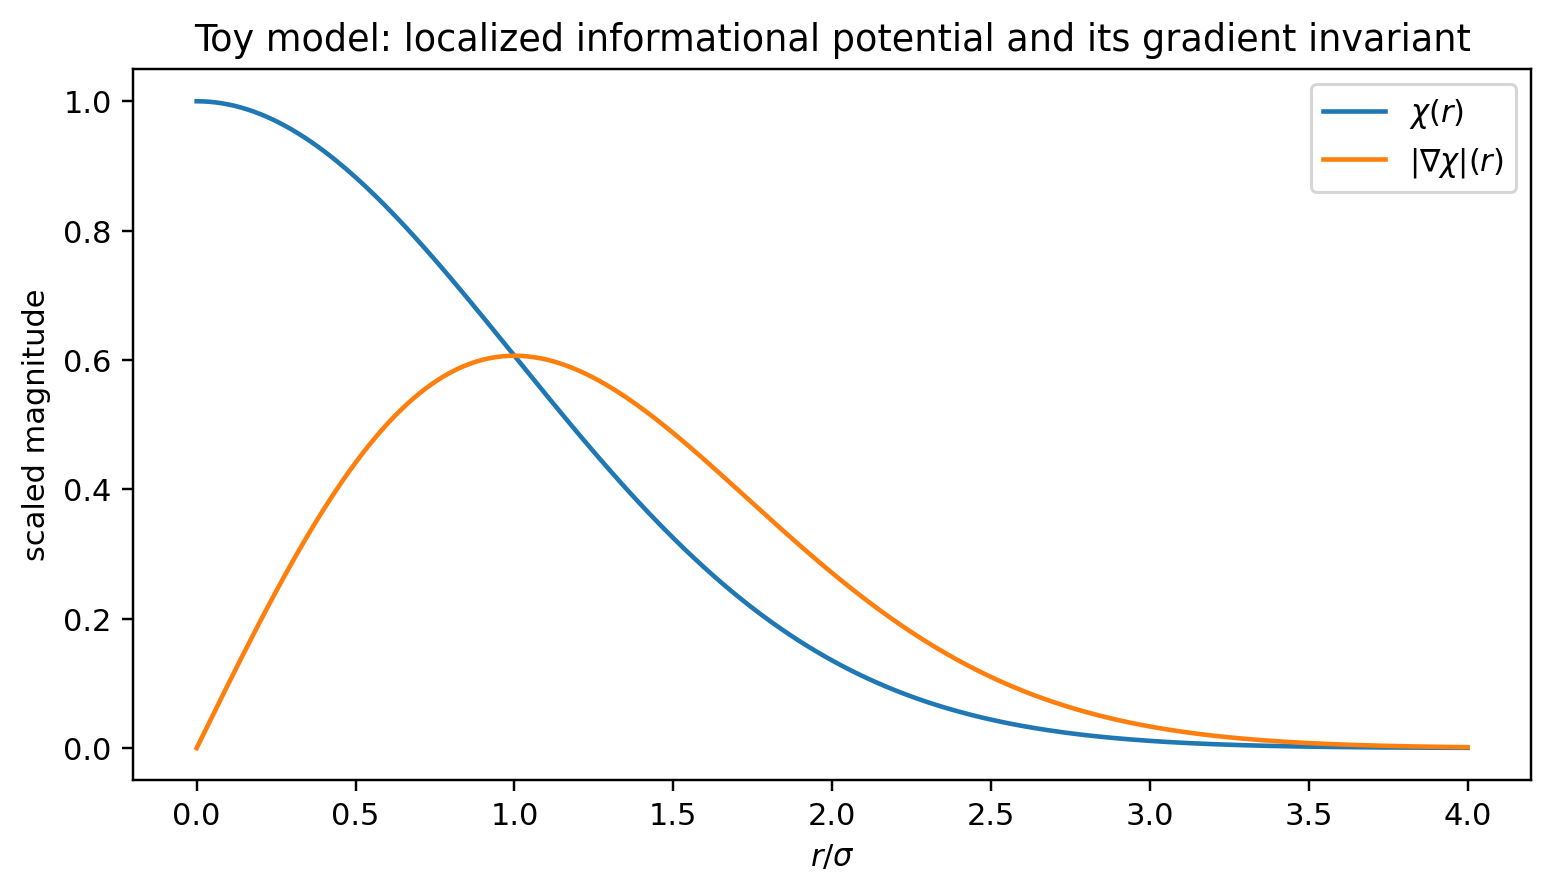
\includegraphics[width=0.9\linewidth]{fig_sst66_v2_04_gaussian_profiles.png}
            \caption{Toy continuous profile: localized $\chi(r)$ and the associated gradient magnitude $|\nabla\chi|(r)$, illustrating where gradient-based clock-rate functionals peak (typically around $r\sim\sigma$).}
            \label{fig:gaussian_profiles}
        \end{figure}

    \subsection{Discrete 2D lattice model with imprint production}
        Let $(i,j)$ index a square lattice with spacing $a$. Define $\chi_{ij}$ and discrete gradients
        \begin{equation}
            (\nabla_x\chi)_{ij}=\frac{\chi_{i+1,j}-\chi_{i,j}}{a},\quad
        (\nabla_y\chi)_{ij}=\frac{\chi_{i,j+1}-\chi_{i,j}}{a}.
        \end{equation}
        Update $\chi$ by a production-diffusion rule
        \begin{equation}
            \chi_{ij}^{(n+1)}=\chi_{ij}^{(n)}+\Delta t\left[\sigma_{ij}+\kappa(\Delta_d\chi)_{ij}^{(n)}\right],
            \label{eq:update}
        \end{equation}
        where $\sigma_{ij}\ge 0$ is an imposed ``imprint'' source and $\Delta_d$ is the 5-point Laplacian. This realizes monotone accumulation when $\sigma_{ij}$ dominates, and relaxation/smoothing when diffusion dominates \cite{LeVeque2002_FVM,Press2007_NR}.

        \begin{figure}[t]
            \centering
            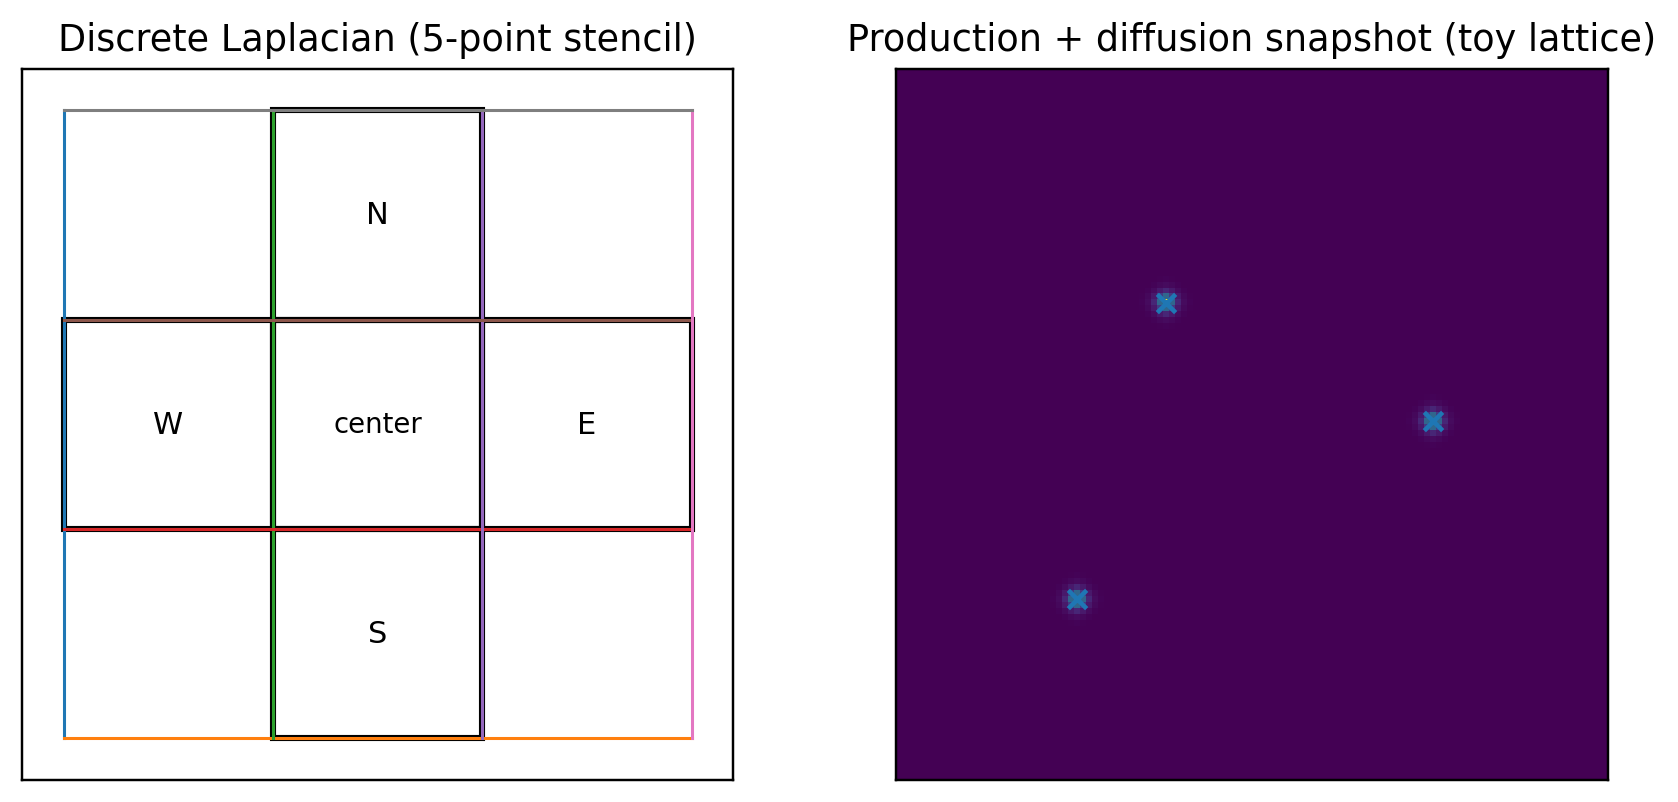
\includegraphics[width=\linewidth]{fig_sst66_v2_05_lattice_stencil_and_snapshot.png}
            \caption{Discrete toy model components. Left: 5-point Laplacian stencil used in the production–diffusion update. Right: example snapshot of $\chi_{ij}$ under localized sources and diffusion (schematic).}
            \label{fig:lattice_stencil_snapshot}
        \end{figure}

    \subsection{Discrete ``curl'' and the need for a rotational component}
        Define a discrete curl of the gradient field. For a pure gradient construction, the discrete curl is (up to numerical error) zero on simply connected regions. Nonzero curl can appear from:
        \begin{enumerate}[label=(\roman*)]
\item defects (cuts, missing nodes, branch points),
\item non-commuting update operators,
\item adding a rotational component (discrete connection) explicitly.
        \end{enumerate}
        This matches the continuum integrability logic and supports the decomposition $\tua=\nabla\chi + A$.

    \subsection{Reference pseudocode}
        \begin{lstlisting}[language=Python,label={lst:lstlisting}]
# 2D lattice informational-time toy simulation (schematic)
import numpy as np

# parameters (choose as needed)
N_steps = 1000
dt = 1e-3
a = 1.0
kappa = 0.1

# fields (example shapes)
Nx, Ny = 128, 128
chi = np.zeros((Nx, Ny))
sigma = np.zeros((Nx, Ny))  # imprint/source term (>=0)

def laplacian(Z):
    # 5-point Laplacian with periodic BC (for simplicity)
    return (np.roll(Z, 1, 0) + np.roll(Z, -1, 0) +
            np.roll(Z, 1, 1) + np.roll(Z, -1, 1) - 4*Z) / (a*a)

for step in range(N_steps):
    # update chi with production + diffusion
    chi = chi + dt*(sigma + kappa*laplacian(chi))

    # forward differences for gradients
    Tx = (np.roll(chi, -1, 0) - chi) / a
    Ty = (np.roll(chi, -1, 1) - chi) / a

    # monitor invariants
    grad2 = Tx**2 + Ty**2
    # curl would be ~0 for pure gradient unless defects/connection are added
        \end{lstlisting}


    \section{Medium-based ``swirl-clock'' mapping}
    \label{sec:clockmap}
    This section introduces a constitutive mapping from a time potential $\chi$ to a clock-rate factor. It is presented as an \emph{analogue/medium model}, not as a derived consequence of GR.

    \subsection{Clock-rate factor and characteristic speed}
        Assume a class of clocks whose intrinsic rate depends on an internal transverse motion scale $v_\perp(x)$ and a characteristic speed $\vnorm$ (a medium parameter):
        \begin{equation}
            dt(x)=dt_\infty\, S_{\!\boldsymbol{\circlearrowleft}}(x),
            \qquad
            S_{\!\boldsymbol{\circlearrowleft}}(x)=\sqrt{1-\frac{v_\perp(x)^2}{\vnorm^2}}.
            \label{eq:clock_factor}
        \end{equation}
        If $\vnorm=c$, \eqref{eq:clock_factor} resembles standard Lorentz time dilation. If $\vnorm\neq c$, it represents an analogue kinematics (as in acoustic metrics where $c$ is replaced by a sound speed) \cite{Unruh1981_SonicBH,Visser1998_Acoustic}.

    \subsection{Linking $v_\perp$ to the time potential}
        A minimal gradient-based closure is
        \begin{equation}
            \frac{v_\perp(x)^2}{\vnorm^2} := \gamma_1\,\ell^2 \|\nabla\chi(x)\|^2 + \gamma_2\,\ell^4 (\nabla_a\nabla_b\chi)(\nabla^a\nabla^b\chi)+\cdots,
            \label{eq:vperp_closure}
        \end{equation}
        where $\ell$ is an interaction length scale (set by clock physics) and $\gamma_i$ are dimensionless couplings to be fit or bounded experimentally. This guarantees dimensional consistency: $\|\nabla\chi\|$ has units s/m, so $\ell^2\|\nabla\chi\|^2$ is dimensionless.

        Expanding \eqref{eq:clock_factor} for small gradients yields
        \begin{equation}
            S_{\!\boldsymbol{\circlearrowleft}}(x)\approx 1-\frac{1}{2}\gamma_1\,\ell^2\|\nabla\chi(x)\|^2+\mathcal{O}(\|\nabla\chi\|^4).
            \label{eq:clock_expand}
        \end{equation}
        This produces explicit predictions for differential clock rates in terms of $\chi$-invariants.

    \subsection{If non-integrable time exists: holonomy-induced offsets}
        If $\tua=\partial_a\chi + A_a$, loop offsets \eqref{eq:stokes} predict a purely geometric-like contribution to time comparisons:
        \begin{equation}
            \Delta\tau_{\rm loop}=\oint A_a\,dx^a = \int_{\Sigma}\Omab\,d\Sigma^{ab}.
            \label{eq:holonomy_clock}
        \end{equation}
        This is structurally analogous to gauge holonomy and can be tested by transporting synchronized clocks around closed loops (or by comparing phases in closed-loop interferometry) \cite{AharonovBohm1959_AB,Nakahara2003_Geometry}.

    \section{Observational program: falsifiable signatures}
    \subsection{Clock networks and gradient-sensitive desynchronization}
        Consider two clocks at $x_1,x_2$ exchanging signals and compared to a common coordinate time $t_{\rm ref}$. A generic prediction is
        \begin{equation}
            \frac{\Delta f}{f}
            \;=\;
            a_1\Big(\|\nabla\chi(x_2)\|^2-\|\nabla\chi(x_1)\|^2\Big)
            + a_2\Big(\mathcal{I}_2-\mathcal{I}_1\Big)
            + \cdots,
            \label{eq:freqshift}
        \end{equation}
        where $\mathcal{I}$ denotes a second-derivative invariant (e.g., $(\nabla\nabla\chi)^2$) and the $a_i$ are parameters determined by the clock physics. Modern optical clock networks can reach sensitivities where extremely small potential differences are measurable in GR contexts \cite{Ludlow2015_OpticalClocks}.

        A key discriminator from standard GR redshift is \emph{dependence on gradients and higher derivatives} rather than solely on gravitational potential (metric component). Any statistically significant residual correlated with $\|\nabla\chi\|$ after accounting for known GR/systematic effects would support an informational/medium extension.

    \subsection{Long-baseline quantum coherence distribution}
        Neukart suggests that entanglement-based timekeeping may probe informational curvature \cite{Neukart2026_InfoTime}. Operationally, phase coherence distributed across regions with varying $\chi$ may accrue an additional contribution. In the non-integrable case,
        \begin{equation}
            \Delta\varphi_{\rm excess} \propto \oint \tua\,dx^a = \oint A_a\,dx^a,
            \label{eq:phase_holonomy}
        \end{equation}
        suggesting a loop-dependent phase/time anomaly akin to a topological effect. Quantum metrology and clock-network proposals provide concrete architectures for such tests \cite{Giovannetti2011_Metrology,Komar2014_ClockNetwork}.

    \subsection{Minimal ``yes/no'' experiment}
        A minimal falsifier (conceptual):
        \begin{enumerate}[label=(\alph*)]
\item Prepare three clocks $C_1,C_2,C_3$ and synchronize pairwise in a baseline configuration.
\item Transport one clock around two distinct closed loops in opposite orientations while controlling standard environmental effects.
\item Compare final offsets. In integrable time ($A_a=0$), the net loop offset must vanish within experimental error; in non-integrable time, the offset can depend on loop orientation and enclosed ``time curvature'' \eqref{eq:holonomy_clock}.
        \end{enumerate}
        The crucial point is \emph{path dependence}: GR proper time depends on worldline, but holonomy here produces an additional loop functional tied to $\Omab$.

        \begin{figure}[t]
            \centering
            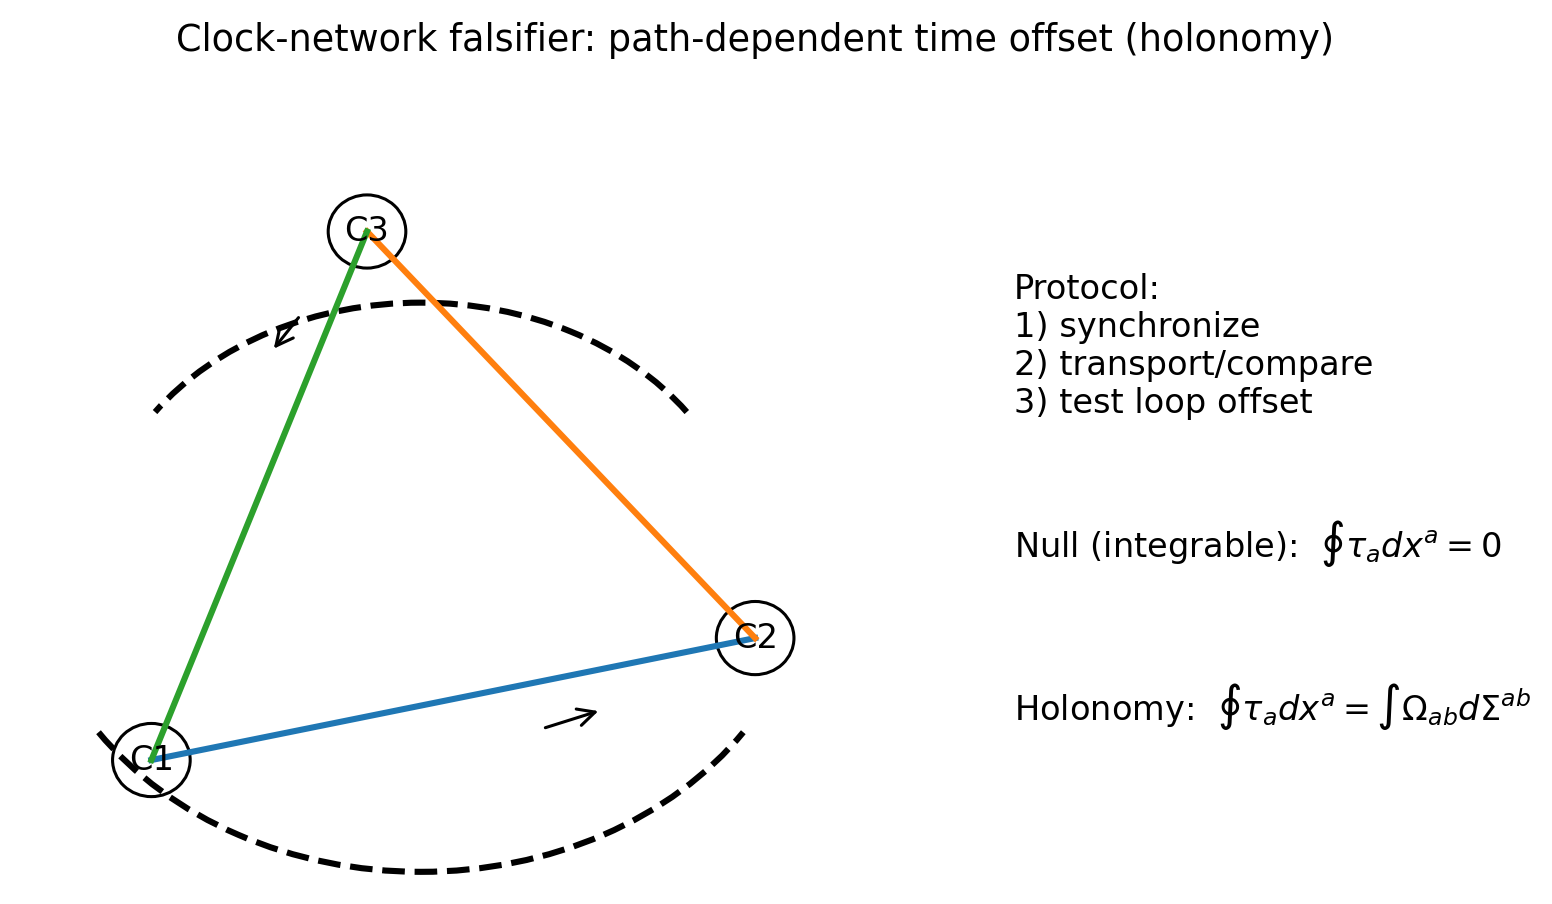
\includegraphics[width=\linewidth]{fig_sst66_v2_06_clock_network_falsifier.png}
            \caption{Clock-network falsifier for holonomy. A triangular network supports two oppositely oriented loops; integrable time predicts zero loop offset, while non-integrable time predicts a loop functional tied to $\Omega_{ab}$.}
            \label{fig:clock_network_falsifier}
        \end{figure}

    \section{Discussion}
    The informational-gradient ansatz provides a compact language for local temporal direction. Making it physically meaningful requires:
    \begin{itemize}
        \item an explicit calibration from information to seconds ($\nu_I$),
        \item an explicit stance on integrability (gradient time vs connection-augmented time),
        \item a covariant coupling to geometry (preferably via stress--energy rather than direct Hessian identification),
        \item an observational program distinguishing gradient/twist signatures from GR and systematics.
    \end{itemize}
    Hessian-metric ideas are conceptually attractive but must address Lorentzian signature and covariance; information geometry offers tools but is not automatically a spacetime theory.

    Medium/analogue mappings (e.g., characteristic speed $\vnorm$) are mathematically legitimate and experimentally useful, but they constitute additional physics assumptions \cite{Unruh1981_SonicBH,Visser1998_Acoustic}. Whether $\vnorm$ equals $c$ is an empirical question, not a convention.

    \section{Conclusion}
    We developed a self-contained effective theory for informational time as a local field: dimensional closure via $\chi=\Sinfo/\nu_I$, integrability clarified through $\tua=\partial_a\chi$ vs $\tua=\partial_a\chi+A_a$ with measurable holonomy, and a conservative covariant coupling to GR. Toy models and simulations were provided, and falsifiable signatures were identified in clock networks and quantum coherence distribution. A medium-based swirl-clock mapping was presented as a constitutive option compatible with analogue-gravity methodology.

    \appendix
    \section{Units and dimensional analysis}
    $\Sinfo$ is dimensionless (nats). Then:
    \[
        [\partial_a \Sinfo]=\mathrm{m}^{-1},\qquad
        [\nu_I]=\mathrm{s}^{-1},\qquad
        [\chi]=\mathrm{s},\qquad
        [\partial_a\chi]=\mathrm{s/m}.
    \]
    The gradient invariants used in \eqref{eq:vperp_closure} are dimensionless when multiplied by suitable powers of a length scale $\ell$.

    \section{Integrability: closed vs exact one-forms}
    On a simply-connected domain, every closed one-form is exact (Poincar\'e lemma) \cite{BottTu1982_DiffForms,Frankel2011_GeometryPhysics}. Thus if $\nabla_{[a}\tua_{b]}=0$ and the domain is simply connected, there exists a scalar $\chi$ such that $\tua=\partial_a\chi$. Nontrivial holonomy requires either (i) non-simply-connected topology, (ii) singularities/defects, or (iii) an explicit connection $A_a$.

    \begin{thebibliography}{99}

        \bibitem{Neukart2026_InfoTime}
        F.~Neukart, 2026,
        \textit{The Geometry and Flow of Informational Time},
        Universe \textbf{12}(1):2.
        doi:10.3390/universe12010002.

        \bibitem{Wald1984_GR}
        R.~M.~Wald, 1984,
        \textit{General Relativity},
        University of Chicago Press.

        \bibitem{DeWitt1967_Canonical}
        B.~S.~DeWitt, 1967,
        \textit{Quantum Theory of Gravity. I. The Canonical Theory},
        Phys.\ Rev.\ \textbf{160}, 1113--1148.
        doi:10.1103/PhysRev.160.1113.

        \bibitem{Isham1993_ProblemTime}
        C.~J.~Isham, 1993,
        \textit{Canonical Quantum Gravity and the Problem of Time},
        in \textit{Integrable Systems, Quantum Groups, and Quantum Field Theories},
        NATO ASI Series C, Springer, Dordrecht.
        (permalink: Springer proceedings volume).

        \bibitem{Kuchar1992_TimeInterp}
        K.~V.~Kucha\v{r}, 1992,
        \textit{Time and Interpretations of Quantum Gravity},
        Proc.\ 4th Canadian Conf.\ on GR and Relativistic Astrophysics,
        World Scientific.
        (permalink: World Scientific proceedings).

        \bibitem{PageWootters1983_Evolution}
        D.~N.~Page and W.~K.~Wootters, 1983,
        \textit{Evolution without evolution: Dynamics described by stationary observables},
        Phys.\ Rev.\ D \textbf{27}, 2885--2892.
        doi:10.1103/PhysRevD.27.2885.

        \bibitem{Rovelli1991_TimeHypothesis}
        C.~Rovelli, 1991,
        \textit{Time in quantum gravity: An hypothesis},
        Phys.\ Rev.\ D \textbf{43}, 442--456.
        doi:10.1103/PhysRevD.43.442.

        \bibitem{Lebowitz1993_Boltzmann}
        J.~L.~Lebowitz, 1993,
        \textit{Boltzmann's entropy and time's arrow},
        Physics Today \textbf{46}(9), 32--38.
        doi:10.1063/1.881363.

        \bibitem{ConnesRovelli1994_ThermalTime}
        A.~Connes and C.~Rovelli, 1994,
        \textit{Von Neumann algebra automorphisms and time-thermodynamics relation in generally covariant quantum theories},
        Class.\ Quant.\ Grav.\ \textbf{11}, 2899--2918.
        doi:10.1088/0264-9381/11/12/007.

        \bibitem{Jacobson1995_ThermoSpacetime}
        T.~Jacobson, 1995,
        \textit{Thermodynamics of spacetime: The Einstein equation of state},
        Phys.\ Rev.\ Lett.\ \textbf{75}, 1260--1263.
        doi:10.1103/PhysRevLett.75.1260.

        \bibitem{Verlinde2011_Entropic}
        E.~P.~Verlinde, 2011,
        \textit{On the Origin of Gravity and the Laws of Newton},
        JHEP \textbf{04}, 029.
        doi:10.1007/JHEP04(2011)029.

        \bibitem{Amari2016_InfoGeometry}
        S.-I.~Amari, 2016,
        \textit{Information Geometry and Its Applications},
        Springer.
        doi:10.1007/978-4-431-55978-8.

        \bibitem{CoverThomas2006_InfoTheory}
        T.~M.~Cover and J.~A.~Thomas, 2006,
        \textit{Elements of Information Theory} (2nd ed.),
        Wiley.

        \bibitem{BottTu1982_DiffForms}
        R.~Bott and L.~W.~Tu, 1982,
        \textit{Differential Forms in Algebraic Topology},
        Springer.
        doi:10.1007/978-1-4757-3951-0.

        \bibitem{Frankel2011_GeometryPhysics}
        T.~Frankel, 2011,
        \textit{The Geometry of Physics: An Introduction} (3rd ed.),
        Cambridge University Press.

        \bibitem{Nakahara2003_Geometry}
        M.~Nakahara, 2003,
        \textit{Geometry, Topology and Physics} (2nd ed.),
        Taylor \& Francis.

        \bibitem{AharonovBohm1959_AB}
        Y.~Aharonov and D.~Bohm, 1959,
        \textit{Significance of Electromagnetic Potentials in the Quantum Theory},
        Phys.\ Rev.\ \textbf{115}, 485--491.
        doi:10.1103/PhysRev.115.485.

        \bibitem{Unruh1981_SonicBH}
        W.~G.~Unruh, 1981,
        \textit{Experimental black-hole evaporation?},
        Phys.\ Rev.\ Lett.\ \textbf{46}, 1351--1353.
        doi:10.1103/PhysRevLett.46.1351.

        \bibitem{Visser1998_Acoustic}
        M.~Visser, 1998,
        \textit{Acoustic black holes: Horizons, ergospheres and Hawking radiation},
        Class.\ Quant.\ Grav.\ \textbf{15}, 1767--1791.
        doi:10.1088/0264-9381/15/6/024.

        \bibitem{LeVeque2002_FVM}
        R.~J.~LeVeque, 2002,
        \textit{Finite Volume Methods for Hyperbolic Problems},
        Cambridge University Press.

        \bibitem{Press2007_NR}
        W.~H.~Press, S.~A.~Teukolsky, W.~T.~Vetterling, and B.~P.~Flannery, 2007,
        \textit{Numerical Recipes: The Art of Scientific Computing} (3rd ed.),
        Cambridge University Press.

        \bibitem{Giovannetti2011_Metrology}
        V.~Giovannetti, S.~Lloyd, and L.~Maccone, 2011,
        \textit{Advances in quantum metrology},
        Nature Photonics \textbf{5}, 222--229.
        doi:10.1038/nphoton.2011.35.

        \bibitem{Komar2014_ClockNetwork}
        P.~K\'om\'ar et al., 2014,
        \textit{A quantum network of clocks},
        Nature Physics \textbf{10}, 582--587.
        doi:10.1038/nphys3000.

        \bibitem{Ludlow2015_OpticalClocks}
        A.~D.~Ludlow, M.~M.~Boyd, J.~Ye, E.~Peik, and P.~O.~Schmidt, 2015,
        \textit{Optical atomic clocks},
        Rev.\ Mod.\ Phys.\ \textbf{87}, 637--701.
        doi:10.1103/RevModPhys.87.637.

    \end{thebibliography}

\end{document}